
\documentclass[11pt]{article}
\usepackage[a4paper,margin=1in]{geometry}
\usepackage{amsmath,amssymb,amsthm,mathtools,tikz}
\usepackage{subcaption}
\usepackage{enumitem}

\newtheorem{theorem}{Theorem}
\newtheorem{lemma}{Lemma}
\newtheorem{proposition}{Proposition}
\newtheorem{corollary}{Corollary}
\newtheorem{remark}{Remark}



\begin{document}
For $\alpha=\frac12$, the generalized approximation ratio is $\lambda(\frac12)=\frac43$.
The variable values for this value of $\alpha$ are $\frac{u}{m}=\frac13$ and $p=3$.

An instance for which this approximation bound is tight, is for example: 

\begin{figure}[ht]
\centering
\begin{subfigure}[t]{0.47\textwidth}
\centering
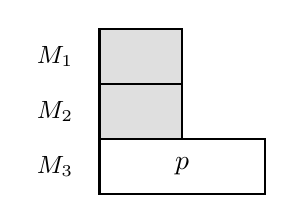
\begin{tikzpicture}[
    x=0.7cm,
    y=0.7cm,
    job/.style={
        draw,
        thick,
        fill=white,
        font=\small
    },
    machine/.style={font=\small}
]

% ------------------------------------------------
% Template idea:
% row      = displayed vertical row in the picture
% machine  = actual machine label shown on the left
%
% Use \machinerow{row}{machine label}
% Use \dotsrow{row}
% Use \jobblock{row}{start}{length}{job label}
% Use \jobblock[gray!25]{row}{start}{length}{job label} for shading
% ------------------------------------------------

\newcommand{\machinerow}[2]{
    \node[machine, anchor=east] at (-0.3,-#1+0.5) {$M_{#2}$};
}

\newcommand{\dotsrow}[1]{
    \foreach \dy in {-0.18,0,0.18} {
        \fill (-0.6,{-#1+0.5+\dy}) circle[radius=0.025];
        \fill (2,{-#1+0.5+\dy}) circle[radius=0.025];
    }
}

\newcommand{\jobblock}[5][white]{
    \draw[job, fill=#1] (#3,-#2) rectangle ++(#4,1);
    \node at ({#3 + #4/2},{-#2 + 0.5}) {$#5$};
}

% Displayed machine rows
\machinerow{1}{1}
\machinerow{2}{2}
\machinerow{3}{3}


% Example jobs
\jobblock[gray!25]{1}{0}{1.5}{}
\jobblock[gray!25]{2}{0}{1.5}{}
\jobblock{3}{0}{3}{p}


\end{tikzpicture}

\caption{$S_{OPT}$}
\label{fig:instance-43-opt}
\end{subfigure}
\hfill
\begin{subfigure}[t]{0.47\textwidth}
\centering
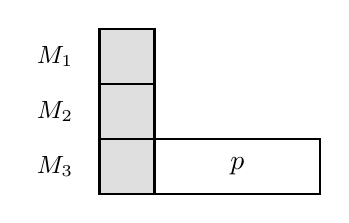
\begin{tikzpicture}[
    x=0.7cm,
    y=0.7cm,
    job/.style={
        draw,
        thick,
        fill=white,
        font=\small
    },
    machine/.style={font=\small}
]

% ------------------------------------------------
% Template idea:
% row      = displayed vertical row in the picture
% machine  = actual machine label shown on the left
%
% Use \machinerow{row}{machine label}
% Use \dotsrow{row}
% Use \jobblock{row}{start}{length}{job label}
% Use \jobblock[gray!25]{row}{start}{length}{job label} for shading
% ------------------------------------------------

\newcommand{\machinerow}[2]{
    \node[machine, anchor=east] at (-0.3,-#1+0.5) {$M_{#2}$};
}

\newcommand{\dotsrow}[1]{
    \foreach \dy in {-0.18,0,0.18} {
        \fill (-0.6,{-#1+0.5+\dy}) circle[radius=0.025];
        \fill (2,{-#1+0.5+\dy}) circle[radius=0.025];
    }
}

\newcommand{\jobblock}[5][white]{
    \draw[job, fill=#1] (#3,-#2) rectangle ++(#4,1);
    \node at ({#3 + #4/2},{-#2 + 0.5}) {$#5$};
}

% Displayed machine rows
\machinerow{1}{1}
\machinerow{2}{2}
\machinerow{3}{3}


% Example jobs
\jobblock[gray!25]{1}{0}{1}{}
\jobblock[gray!25]{2}{0}{1}{}
\jobblock[gray!25]{3}{0}{1}{}
\jobblock{3}{1}{3}{p}


\end{tikzpicture}

\caption{$S_{\mathrm{WSPT}}$}
\label{fig:instance-43-lrf}
\end{subfigure}
\caption{Gray blocks mark the short jobs}
\label{fig:instance-43-ratio}
\end{figure}

\end{document}
